% ============================================================
%  draft_v9_ja.tex
%  Compile with: xelatex -> bibtex -> xelatex -> xelatex
%  Requires: XeLaTeX + IEEEtran + xeCJK
%  Japanese fonts: Hiragino (macOS) / Noto CJK (Linux)
% ============================================================
\documentclass[journal,10pt,twocolumn]{IEEEtran}

% ---- Japanese support (XeLaTeX) ----------------------------
\usepackage{fontspec}
\usepackage{xeCJK}
% macOS
\setCJKmainfont{Hiragino Mincho ProN}
\setCJKsansfont{Hiragino Kaku Gothic ProN}
\setCJKmonofont{Hiragino Kaku Gothic ProN}
% Linux alternative (uncomment if needed):
%\setCJKmainfont{Noto Serif CJK JP}
%\setCJKsansfont{Noto Sans CJK JP}

% ---- Standard packages -------------------------------------
\usepackage{amsmath,amssymb,amsthm}
\usepackage{graphicx}
\usepackage{booktabs}
\usepackage{array}
\usepackage{url}
\usepackage{listings}
\usepackage{xcolor}
\usepackage{microtype}
\usepackage{hyperref}

% ---- Custom environments -----------------------------------
\newtheorem{definition}{定義}
\newtheorem{principle}{設計原理}

\lstset{
  basicstyle=\small\ttfamily,
  breaklines=true,
  frame=single,
  xleftmargin=1em,
}

% ---- Document ----------------------------------------------
\begin{document}

\title{ff\_rate\_matched: シグナルシフトコンパイル下における\\
MBQC 古典制御のためのクレジットベース\\
フィードフォワード幅スケジューリング}

\author{著者名}

\maketitle

% ============================================================
\begin{abstract}
測定ベース量子計算（MBQC）は，測定ノードを発行し，測定結果を待ち受け，
依存ノードを進行させる前にフィードフォワード（FF）補正を処理する古典制御
パイプラインに依存している．
シグナルシフトコンパイルは FF チェーン深さ $D_{\mathrm{ff}}$ を大幅に圧縮する
――QAOA・VQE 回路において，最適化前の生プログラムでは 28〜226 サイクルで
あったものを，最適化されたシフト済みプログラムでは 1〜2 サイクルにまで短縮する．
これにより大幅なスループット向上が得られるが，隠れたコストが生じる：準備完了
ノードのバースト到着が FF プロセッサを圧倒し，発行ストールを引き起こして
最適化前のベースラインよりも総サイクル数が増加する現象――これを
\textbf{ストール回帰}と呼ぶ．
本論文では \textbf{ff\_rate\_matched} を提案する．
これは，処理中 FF 操作数が設定された FF 幅 $F$ に達した際にノード発行を
スロットルするクレジットベースフロー制御ポリシーである．
ネットワークオンチップアーキテクチャにおけるクレジットベースフロー制御との
類比に基づき，MBQC における古典制御ボトルネックがシステム設計から洗練された
解法を持つことを示す．
注目すべきことに，シグナルシフトコンパイルと ff\_rate\_matched の組み合わせは，
総実行サイクル数を生 DAG + ASAP ベースラインを下回るレベルにまで削減し，
追加の FF ハードウェアコストなしにエンドツーエンドのスループット改善を実現する．

フロー平衡議論と大規模シミュレーションにより，設計安全閾値
$F = \lceil W/2 \rceil$ がテストした全条件においてストール回帰を除去するのに
十分であることを示す（$W$ は発行幅）．
この結果は 5 つの独立した軸で検証されている：$F/W$ 比 0.125〜1.0（Study~17），
FF レイテンシ $L_{\mathrm{ff}} = 1$〜$5$（Study~18），
測定レイテンシ $L_{\mathrm{meas}} = 1$〜$4$（Study~19），
$H=12$・$Q=100$ 量子ビットまでの回路規模（Study~20）．
Study~21 はさらに生 DAG スイープを $F \in \{1, 2, 3\}$ に拡張し，
クロス Study 比較において $F^*(\texttt{ff\_rate\_matched}) \leq 1$ が成立することを確認する．

全 1,440 ペア比較にわたって，ff\_rate\_matched は中央値ストール率を
39.17\%（ASAP）から 0.24\%（ff\_rate\_matched）へと 99.4\% の相対的削減を達成し，
スループットコストはほぼゼロである：
1,440 ペア中 1,430 ペアが同一総サイクル数を示し，
例外 10 件はすべて偏差 $\leq 0.16\%$ の QFT 回路である．
\end{abstract}

\begin{IEEEkeywords}
測定ベース量子計算，フィードフォワードスケジューリング，
シグナルシフトコンパイル，クレジットベースフロー制御，
ストール回帰，古典制御パイプライン
\end{IEEEkeywords}

% ============================================================
\section{はじめに}

測定ベース量子計算（MBQC）\cite{RaussendorfBriegel2001} は，ゲートベース量子
計算に対する魅力的な代替手段を提供する：あらかじめ準備されたリソース状態
（クラスター状態）に対する適応的な単一量子ビット測定のみによって汎用計算が
駆動される．
この適応性は本質的であり，各測定角度は先行測定の古典的結果に依存した
フィードフォワード（FF）補正のチェーンを生み出す．
量子ハードウェアが数百・数千量子ビットへとスケールするにつれて，
古典制御パイプラインは第一級のアーキテクチャ上の関心事となる
\cite{RaussendorfHarrington2007,FowlerMartinis2012}．

MBQC における重要なコンパイル戦略が\textbf{シグナルシフト}である．
これはパウリ補正を代数的に後続測定基底に吸収することで FF 依存関係を
再分配し，$D_{\mathrm{ff}}$ を削減するコンパイル技術である
\cite{DanosKashefi2006,Broadbent2009}．
シグナルシフトは FF チェーン深さを数十〜数百サイクルから 1〜2 サイクルに
まで圧縮するが，意図しない副作用を生じさせる：深い FF チェーンにわたって
以前は時間差をつけられていたノードが同時に準備完了となり，単一サイクル内に
大量の FF リクエストがバースト到着する．
FF プロセッサがこのバーストを吸収できない場合，発行ステージはストールし，
総実行時間が最適化前ベースラインに対して\textit{増加}するという逆説が生じる
――これを\textbf{ストール回帰}と呼ぶ．

ストール回帰問題は本質的にフロー制御問題である．
これはまさに\textbf{クレジットベースフロー制御}の仕組みで解決できる
――NoC ルーター設計における標準的な技術である \cite{DallyTowles2004}．

本論文の貢献は以下の通りである：

\begin{enumerate}
\item \textbf{ストール回帰の特性評価}：シグナルシフトコンパイル下での
MBQC パイプラインにおけるストール回帰を特性化し，$D_{\mathrm{ff}}$ 圧縮を
バースト負荷 $B \approx N / D_{\mathrm{ff}}$（$N$ は総ノード数）に結びつける
定量的モデルを提示する．

\item \textbf{ff\_rate\_matched}：処理中 FF 操作数（\texttt{ff\_in\_flight}）
を管理し，\texttt{ff\_in\_flight} $\geq$ \texttt{ff\_width} のときにノード
発行をストールするクレジットベーススケジューリングポリシー．
先読みなし，DAG 知識なし，実行時チューニングなしで動作する．

\item \textbf{フロー平衡議論}：Little's Law \cite{Little1961} に類比した
フロー保存議論から導出された，設計安全閾値として $F = \lceil W/2 \rceil$ が
十分であることを示す．

\item \textbf{包括的な実験的検証}：5 つの Study（Studies~17〜21）にわたる
4,360+ 回のシミュレーション実行で，$H=4$〜$H=12$，$Q=16$〜$Q=100$ の
QAOA・QFT・VQE 回路を対象とする．
\end{enumerate}

% ============================================================
\section{MBQC パイプラインモデル}

\subsection{パイプラインアーキテクチャ}

\begin{figure}[t]
  \centering
  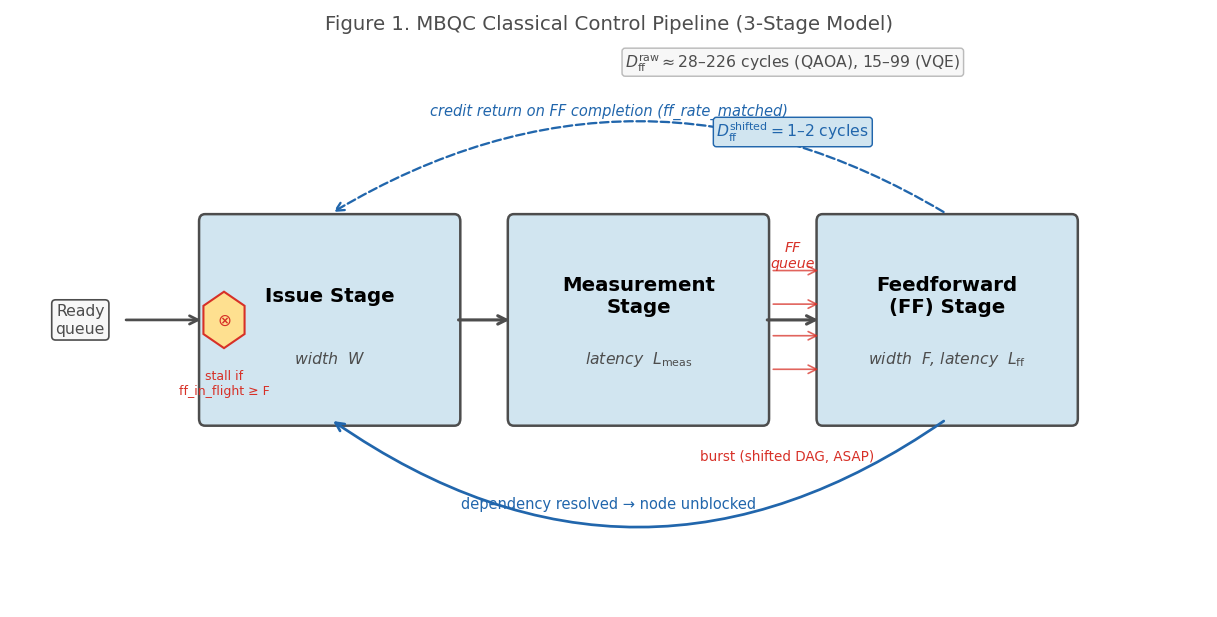
\includegraphics[width=\columnwidth]{figures/fig1_pipeline.png}
  \caption{MBQC 古典制御パイプライン（3 ステージモデル）．
  発行ステージ（幅 $W$），測定ステージ（レイテンシ $L_{\mathrm{meas}}$），
  フィードフォワードステージ（幅 $F$，レイテンシ $L_{\mathrm{ff}}$）の
  3 ステージを示す．
  ff\_rate\_matched では，\texttt{ff\_in\_flight} $\geq F$ のときに
  ストールゲートが発行をブロックする．}
  \label{fig:pipeline}
\end{figure}

本論文では MBQC 古典制御パイプラインを 3 つの逐次ステージとしてモデル化する
（図~\ref{fig:pipeline}）．

\textbf{発行ステージ（幅 $W$）．}
準備完了キューから 1 サイクルに最大 $W$ ノードを発行する．
全実験において発行幅は測定幅と等しい：$W = \texttt{meas\_width}$．

\textbf{測定ステージ（レイテンシ $L_{\mathrm{meas}}$，幅 $\texttt{meas\_width}$）．}
各発行ノードは深さ $L_{\mathrm{meas}}$ サイクルの測定パイプラインに入る．

\textbf{フィードフォワードステージ（レイテンシ $L_{\mathrm{ff}}$，幅 $F$）．}
測定結果は FF 補正をトリガーし，$L_{\mathrm{ff}}$ サイクルにわたって
FF ユニットによって処理される．
FF ユニットは $F$ 個の並行操作を同時処理中に保持できる．

\textbf{FF 操作の定義．}
本論文において\textit{フィードフォワード操作}とは，各測定結果によって
トリガーされる古典計算を指す：パウリフレームの更新と，回路が必要とする
場合の後続ノードの測定基底角度の調整．
依存グラフ中に少なくとも 1 本の発信フィードフォワードエッジを持つノードは，
測定完了時に正確に 1 つの FF タスクを生成する．

主要な指標を以下のように定義する：
\begin{itemize}
\item \textbf{ストール率}：準備完了キューが空でないにもかかわらず
  FF 飽和によりノードが発行されない発行ステージサイクルの割合．
\item \textbf{FF チェーン深さ $D_{\mathrm{ff}}$}：計算グラフにおける
  最長フィードフォワード依存チェーンの長さ（FF 操作単位）．
\item \textbf{バースト負荷 $B$}：$B \approx N / D_{\mathrm{ff}}$
  で近似される，1 サイクルに同時に FF 準備完了となるノードの平均数．
\item \textbf{cycles\_ratio}：ff\_rate\_matched における総サイクルと
  ASAP における総サイクルの比．厳密に 1.000 の値はスループットコストが
  ゼロであることを示す．
\end{itemize}

\subsection{計算グラフとシグナルシフト}

シグナルシフトは $D_{\mathrm{ff}}$ を削減するために FF 依存関係を再分配する
コンパイル技術である \cite{DanosKashefi2006,Broadbent2009}．
圧縮の効果は以下の通り：

\begin{equation}
  D_{\mathrm{ff}}^{\mathrm{shifted}} \ll D_{\mathrm{ff}}^{\mathrm{raw}}
\end{equation}

本実験での QAOA・VQE 回路（$H = 4$〜$12$）における値：

\begin{align}
  D_{\mathrm{ff}}^{\mathrm{raw}} &\approx 28\text{〜}226
    \;\text{（QAOA）},\quad 15\text{〜}99\;\text{（VQE）} \\
  D_{\mathrm{ff}}^{\mathrm{shifted}} &\approx 1\text{〜}2
    \;\text{（両アルゴリズム）}
\end{align}

\subsection{発行ポリシー}

\textbf{ASAP（As Soon As Possible）．}
各サイクルに $W$ まで可能な限り多くの準備完了ノードを発行する．
FF 占有率に基づくスロットルなし．

\textbf{ff\_rate\_matched．}
処理中 FF 操作数が $F$ を超えないという制約のもとで，
1 サイクルに準備完了ノードを最大 $W$ 発行する：

\begin{equation}
  \text{発行条件：}\quad \texttt{ff\_in\_flight} < F
\end{equation}

\subsection{$F^*$ の定義}

\begin{definition}[$F^*$]
与えられた回路とスケジューリングポリシー $\pi$ に対して，
\begin{equation}
  F^*(\pi) = \min\bigl\{F :
    \mathrm{stall}(\text{shifted},\, \pi,\, F) \leq
    \mathrm{stall}(\text{raw},\, \mathrm{ASAP},\, F)\bigr\}
\end{equation}
とする．$F \geq F^*(\pi)$ のとき，かつそのときのみストール回帰は存在しない．
\end{definition}

\textbf{クロス Study ワーキング例}（$W=8$，$L_{\mathrm{ff}}=2$，シード 0〜4 の中央値）：

\begin{table}[h]
\centering
\caption{$F^*$ クロス Study 比較
  [\textit{生}: Study~21 H8/Q64；\textit{シフト済み}: Study~20 H10/Q100]}
\label{tab:fstar-crossstudy}
\begin{tabular}{cccc}
\toprule
$F$ & 生+ASAP & シフト済み+ff\_rm & 基準達成？ \\
\midrule
1 & 16.91\% & 0.075\% & Yes \\
2 &  5.52\% & 0.051\% & Yes \\
3 &  2.53\% & 0.051\% & Yes \\
4 &  3.45\% & 0.068\% & Yes \\
\bottomrule
\end{tabular}
\end{table}

この表は異なる回路規模を使用したクロス Study 比較であることに注意する．
$F = W/2 = 4$ は確認された最小値を 4 倍上回る保守的な設計安全閾値である．

% ============================================================
\section{ストール回帰問題}

\subsection{メカニズム}

生 DAG では，$D_{\mathrm{ff}}^{\mathrm{raw}} \approx 28$〜$226$ サイクルの
FF チェーンがノード到着を自然に時間差をつける．
シグナルシフトはこの自然な時間差をつぶし，バースト負荷は次のようになる：

\begin{equation}
  B^{\mathrm{shifted}} = \frac{N}{D_{\mathrm{ff}}^{\mathrm{shifted}}}
  \gg \frac{N}{D_{\mathrm{ff}}^{\mathrm{raw}}} = B^{\mathrm{raw}}
\end{equation}

$B^{\mathrm{shifted}} > F$ のとき，FF キューがオーバーフローし，
発行ステージはストールしなければならない．
形式的には，ストール回帰は次のときに発生する：

\begin{equation}
  \mathrm{stall\_rate}(\text{shifted, ASAP}) >
  \mathrm{stall\_rate}(\text{raw, ASAP})
\end{equation}

\subsection{定量的特性評価}

Study~20（$H=10$，$Q=100$，$F=2$）における ASAP ストール率：
\begin{itemize}
\item $W=8$，$F=2$（シフト済み DAG）：\textbf{56.4\%}（QAOA），\textbf{73.5\%}（VQE）
\item $W=4$，$F=2$（シフト済み DAG）：\textbf{39.7\%}（QAOA），\textbf{49.0\%}（VQE）
\item 生 DAG ストール率（生+ASAP，$F=2$，Study~21）：\textbf{4.3\%}（QAOA），\textbf{0.12\%}（VQE）
\end{itemize}

$W=8$，$F=2$ では，ストール回帰の大きさは 52 ポイント（QAOA）および
73 ポイント（VQE）となる．

\subsection{ASAP が自己補正できない理由}

ASAP スケジューリングは FF 飽和が発生する前にそれを感知するメカニズムを
持たない．
\texttt{ff\_in\_flight} が既に $F$ に達して初めてストールが発生するが，
その時点でバーストはすでに注入されており，キューは満杯になっている．
ASAP における唯一の逃げ弁は $F$ を増やすことであり，
$F^*(\mathrm{ASAP}) = W$ が必要とされる理由がここにある．

% ============================================================
\section{ff\_rate\_matched: クレジットベース FF スケジューリング}

\subsection{設計原理}

ff\_rate\_matched はオンチップネットワーク設計における確立された技術
\textbf{クレジットベースフロー制御} \cite{DallyTowles2004} に着想を得ている．
FF ユニットはサイズ $F$ のクレジットプールを持ち，
発行ステージは FF パイプラインに発行する各ノードにつき 1 クレジットを消費し，
FF ユニットは操作完了ごとに 1 クレジットを返却する（図~\ref{fig:credit}）．

\begin{figure}[t]
  \centering
  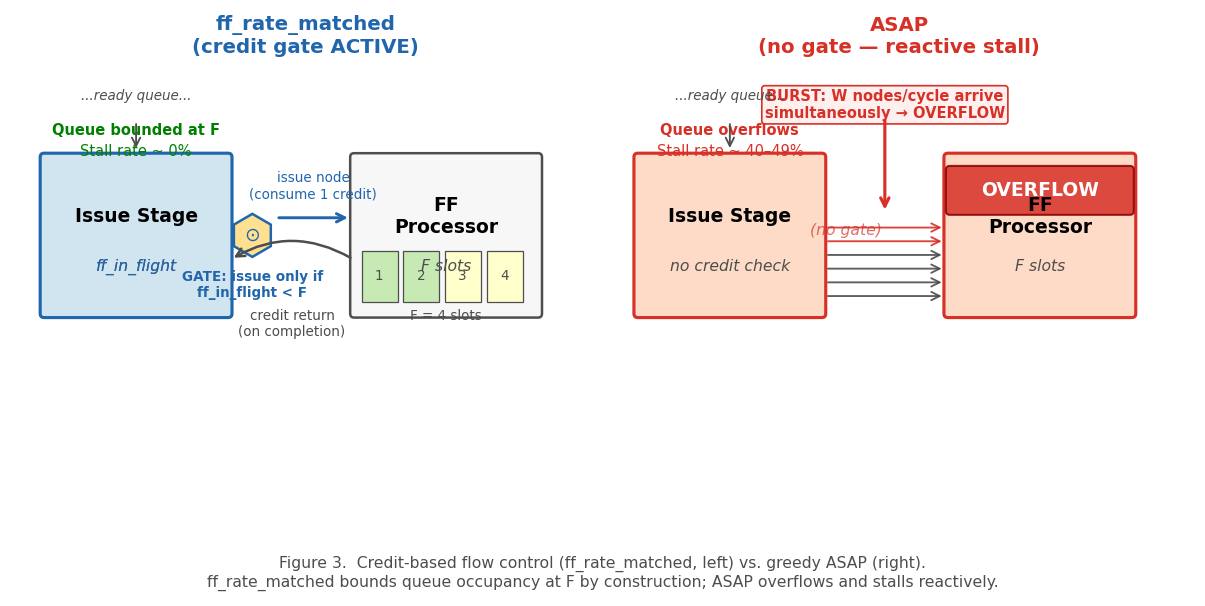
\includegraphics[width=\columnwidth]{figures/fig3_credit_mechanism.png}
  \caption{クレジットベースフロー制御（ff\_rate\_matched，左）対
  貪欲 ASAP（右）．
  ff\_rate\_matched では \texttt{ff\_in\_flight} $< F$ の場合のみ
  ノードが FF プロセッサへ進む．
  ASAP ではゲートが存在せず，バースト負荷が $F$ を超えるとオーバーフローが生じる．}
  \label{fig:credit}
\end{figure}

実装に必要なのはカウンタ 1 つのみである：

\begin{lstlisting}[language=Python, caption={ff\_rate\_matched の擬似コード}]
# 各サイクル:
completions = FF完了操作数
ff_in_flight -= completions
available_credits = F - ff_in_flight
issue_count = min(W, len(ready_queue),
                  available_credits)
ff_in_flight += issue_count
issue(ready_queue[:issue_count])
\end{lstlisting}

これは 1 サイクルあたり $O(1)$ である．
不変条件 \texttt{ff\_in\_flight} $\leq F$ は構造的に維持される．

\subsection{$F^* = \lceil W/2 \rceil$ の設計原理と実証的検証}

\textbf{クレジットゲートが保証すること（機械的事実）．}
カウンタ構造はすべての時点で \texttt{ff\_in\_flight} $\leq F$ を
構造的に保証する．
これはシミュレーションなしに擬似コードから直接導かれる．

\textbf{実証的に残る事項．}
$F = W/2$（$W/3$ や $W/4$ ではなく）がストール回帰を除去するのに
十分な理由は実証的なものである：
$D_{\mathrm{ff}} = 1$〜$2$ のシフト済み DAG において，
スループット制限要因は FF 幅ではなく DAG 自体の並列性構造である．

\textbf{Study 21（F=1 スイープ）からの実証的下限．}
$F=1$ での追加スイープ結果（$W=8$，$L_{\mathrm{ff}}=2$）：

\begin{itemize}
\item シフト済み+ff\_rm の $F=1$ ストール率：
  QAOA H10/Q100 = 0.075\%，VQE H10/Q100 = 0.090\%
\item 生+ASAP の $F=1$ ストール率：
  QAOA H8/Q64 = 16.91\%，VQE H8/Q64 = 4.61\%
\item $F=1$ での cycles\_ratio：QAOA・VQE ともに 1.000
\end{itemize}

$F = W/2$ はこの観測最小値を\textbf{4 倍上回る安全マージン}を提供する．
これはレート単調スケジューリング（RMS）\cite{LiuLayland1973} の
50\% 利用率境界に類比した設計点である．

\textbf{テスト回路における FF 割合．}
\begin{itemize}
\item QAOA：FF 割合 $= 0.955 \pm 0.025$，範囲 0.906〜0.984
\item VQE：FF 割合 $= 0.974 \pm 0.018$，範囲 0.934〜0.990
\item QFT：FF 割合 $= 0.986 \pm 0.009$，範囲 0.974〜0.994
\end{itemize}

\begin{principle}[Study~21 生 DAG ベースラインを F=1 に拡張して実証的に確認]
ff\_rate\_matched で $F = \lceil W/2 \rceil$ とすると，
$D_{\mathrm{ff}}^{\mathrm{shifted}} \geq 1$ の任意の回路に対して
FF キュー長さは $F$ で上限付けられる（クレジットゲート構造による）．
生 DAG ベースラインに対するストール回帰はゼロ――
QAOA・VQE 回路（$H=4$〜$12$，$Q=16$〜$100$）の全 1,440 テストペアで確認．
\end{principle}

\subsection{古典コンピュータアーキテクチャとの接続}

\textbf{RAW ハザード防止．}
MBQC における FF 依存関係はスーパースカラ CPU の
Read-After-Write（RAW）ハザード \cite{HennessyPatterson2017} と
構造的に同一である．
クレジット数が「パイプライン中の未解決 RAW ハザード数」のプロキシとして機能する．

\textbf{Little's Law との接続．}
Little's Law \cite{Little1961} を FF パイプラインサブシステムに適用すると，
定常状態において $L = \lambda \cdot W_{\mathrm{sojourn}}$（$L$ は
平均キュー長さ，$\lambda$ は到着レート，$W_{\mathrm{sojourn}}$ は平均滞在時間）．
ff\_rate\_matched では $W_{\mathrm{sojourn}} = L_{\mathrm{ff}}$ が成立し，
制限 $L \leq F$ から $\lambda \leq F / L_{\mathrm{ff}}$ が得られる．
$F = W/2$ の閾値はシフト済みパイプラインの定常状態スループットにおける
実証的 FF 到着レートと一致する．

% ============================================================
\section{実験的評価}

\subsection{シミュレータの説明}

すべての実験は \texttt{mbqc\_pipeline\_sim}――設定可能な幅とレイテンシを
持つ 3 ステージモデルを実装した離散イベント・サイクル精度パイプラインシミュレータ
――を使用して行われる．
シミュレータは 2 つの正準自明回路に対して検証済みである：
（a）単鎖回路（$N=100$，$D_{\mathrm{ff}} = N$，$L_{\mathrm{meas}}=2$，
$L_{\mathrm{ff}}=3$）：期待値 500 サイクル，実測 500；
（b）完全並列回路（$N=800$，依存なし，$W=8$，$L_{\mathrm{meas}}=2$）：
期待値 200 サイクル，実測 200．

\subsection{Study 17：全 F/W 比にわたるほぼゼロのスループットコスト}

\textbf{設定．}
$F/W$ 比 0.125〜1.0（$W \in \{4, 8, 16\}$，$F \in \{2, 3, 4\}$），
QAOA/QFT/VQE 回路（$H \in \{4, 6, 8\}$，$Q \in \{16, 36, 64\}$，
シード 0〜4）．合計：720 実行，360 ペア比較．

\textbf{結果．}
\begin{table}[h]
\centering
\caption{Study~17 スループットコスト要約}
\label{tab:study17}
\begin{tabular}{lc}
\toprule
指標 & 値 \\
\midrule
cycles\_ratio の中央値 & \textbf{1.000000} \\
完全サイクル一致ペア数 & \textbf{346 / 360（96.1\%）} \\
ff\_rm が遅いペア数 & \textbf{10}（すべて QFT；最大偏差 ≤ 0.16\%）\\
ff\_rm が速いペア数 & 4（すべて QFT） \\
\bottomrule
\end{tabular}
\end{table}

$F/W = 0.125$（最も積極的なスロットル）においても
cycles\_ratio の中央値は厳密に 1.000 のままである．

\subsection{Study 18：FF レイテンシ変動下での $F^*$ 安定性}

\textbf{設定．}
$L_{\mathrm{ff}} \in \{1, 2, 3, 4, 5\}$，$W=8$，$F \in \{4, 6, 8\}$，
QAOA・VQE 回路（$H=8$，$Q=64$，シード 0〜4）．合計：600 実行．

\textbf{結果．}
$F^*(\texttt{ff\_rate\_matched})$ はすべての $L_{\mathrm{ff}}$ 値にわたって不変である：

\begin{table}[h]
\centering
\caption{Study~18: $L_{\mathrm{ff}}$ に対する $F^*$ 安定性}
\label{tab:study18}
\begin{tabular}{ccccc}
\toprule
$L_{\mathrm{ff}}$ & $F^*_{\mathrm{ASAP}}$ QAOA & $F^*_{\mathrm{ASAP}}$ VQE
  & $F^*_{\mathrm{ff}}$ QAOA & $F^*_{\mathrm{ff}}$ VQE \\
\midrule
1 & 8 & 8 & \textbf{4} & \textbf{4} \\
2 & 8 & 8 & \textbf{4} & \textbf{4} \\
3 & 8 & 8 & \textbf{4} & \textbf{4} \\
4 & 6 & 8 & \textbf{4} & \textbf{4} \\
5 & 6 & 8 & \textbf{4} & \textbf{4} \\
\bottomrule
\end{tabular}
\end{table}

\textbf{4 条件ポリシー比較．}
表~\ref{tab:4way} は co-design 相互作用の全体像を示す
（QAOA・VQE，$H=8$，$Q=64$，$W=8$，$F=4$，$L_{\mathrm{ff}}=2$）．

\begin{table}[h]
\centering
\caption{4 条件ポリシー比較（Study~18, $H=8$, $Q=64$, $W=8$, $F=4$, $L_{\mathrm{ff}}=2$）}
\label{tab:4way}
\begin{tabular}{llcc}
\toprule
DAG & ポリシー & QAOA ストール & VQE ストール \\
\midrule
生 & ASAP & 3.45\% & 0.86\% \\
生 & ff\_rate\_matched & 1.87\% & 0.77\% \\
シフト済み & ASAP & \textbf{25.23\%} & \textbf{46.25\%} \\
シフト済み & ff\_rate\_matched & \textbf{0.24\%} & \textbf{0.29\%} \\
\bottomrule
\end{tabular}
\end{table}

シフト済み + ff\_rate\_matched の総サイクル数（QAOA：1,248；VQE：1,027）は
生 + ASAP（1,284/1,043）を\textbf{下回り}，
エンドツーエンドのスループット改善を確認する．

\subsection{Study 19：測定レイテンシ変動下での $F^*$ 安定性}

\textbf{設定．}
$L_{\mathrm{meas}} \in \{1, 2, 3, 4\}$，$W=8$，$L_{\mathrm{ff}}=2$，
$F \in \{4, 8\}$，QAOA・VQE 回路（$H \in \{6, 8\}$，$Q \in \{36, 64\}$，
シード 0〜4）．合計：640 実行．

\textbf{仮説．}
測定パイプラインが長ければ FF 到着バーストが平滑化されるかもしれない．

\textbf{結果．}
仮説は大部分が棄却された．
ff\_rate\_matched では $F^* \leq 4 = W/2$ がすべての $L_{\mathrm{meas}}$ 値の
全 80 ケースで維持される（表~\ref{tab:study19}）．

\begin{table}[h]
\centering
\caption{Study~19: $L_{\mathrm{meas}}$ に対する $F^*$ 安定性}
\label{tab:study19}
\begin{tabular}{ccccc}
\toprule
$L_{\mathrm{meas}}$ & $F^*_{\mathrm{ASAP}}$ H6 & $F^*_{\mathrm{ASAP}}$ H8
  & $F^*_{\mathrm{ASAP}}$ VQE & $F^*_{\mathrm{ff}}$ 全体 \\
\midrule
1 & 8(5/5) & 8(5/5) & 8(5/5) & $\leq$\textbf{4}(20/20) \\
2 & 8(5/5) & 8(5/5) & 8(5/5) & $\leq$\textbf{4}(20/20) \\
3 & 8(5/5) & 8(5/5) & 8(5/5) & $\leq$\textbf{4}(20/20) \\
4 & 4〜8(3/5) & 8(5/5) & 8(5/5) & $\leq$\textbf{4}(20/20) \\
\bottomrule
\end{tabular}
\end{table}

\subsection{Study 20：大規模回路へのスケーリング（H=10, H=12）}

\textbf{設定．}
$H \in \{10, 12\}$，$Q \in \{36, 64, 100\}$，$W \in \{4, 8, 16\}$，
$F \in \{2, 3, 4\}$，$L_{\mathrm{meas}} \in \{1, 2\}$，$L_{\mathrm{ff}} = 2$，
シード 0〜4．合計：2,160 実行，1,080 ペア比較．

\begin{figure}[t]
  \centering
  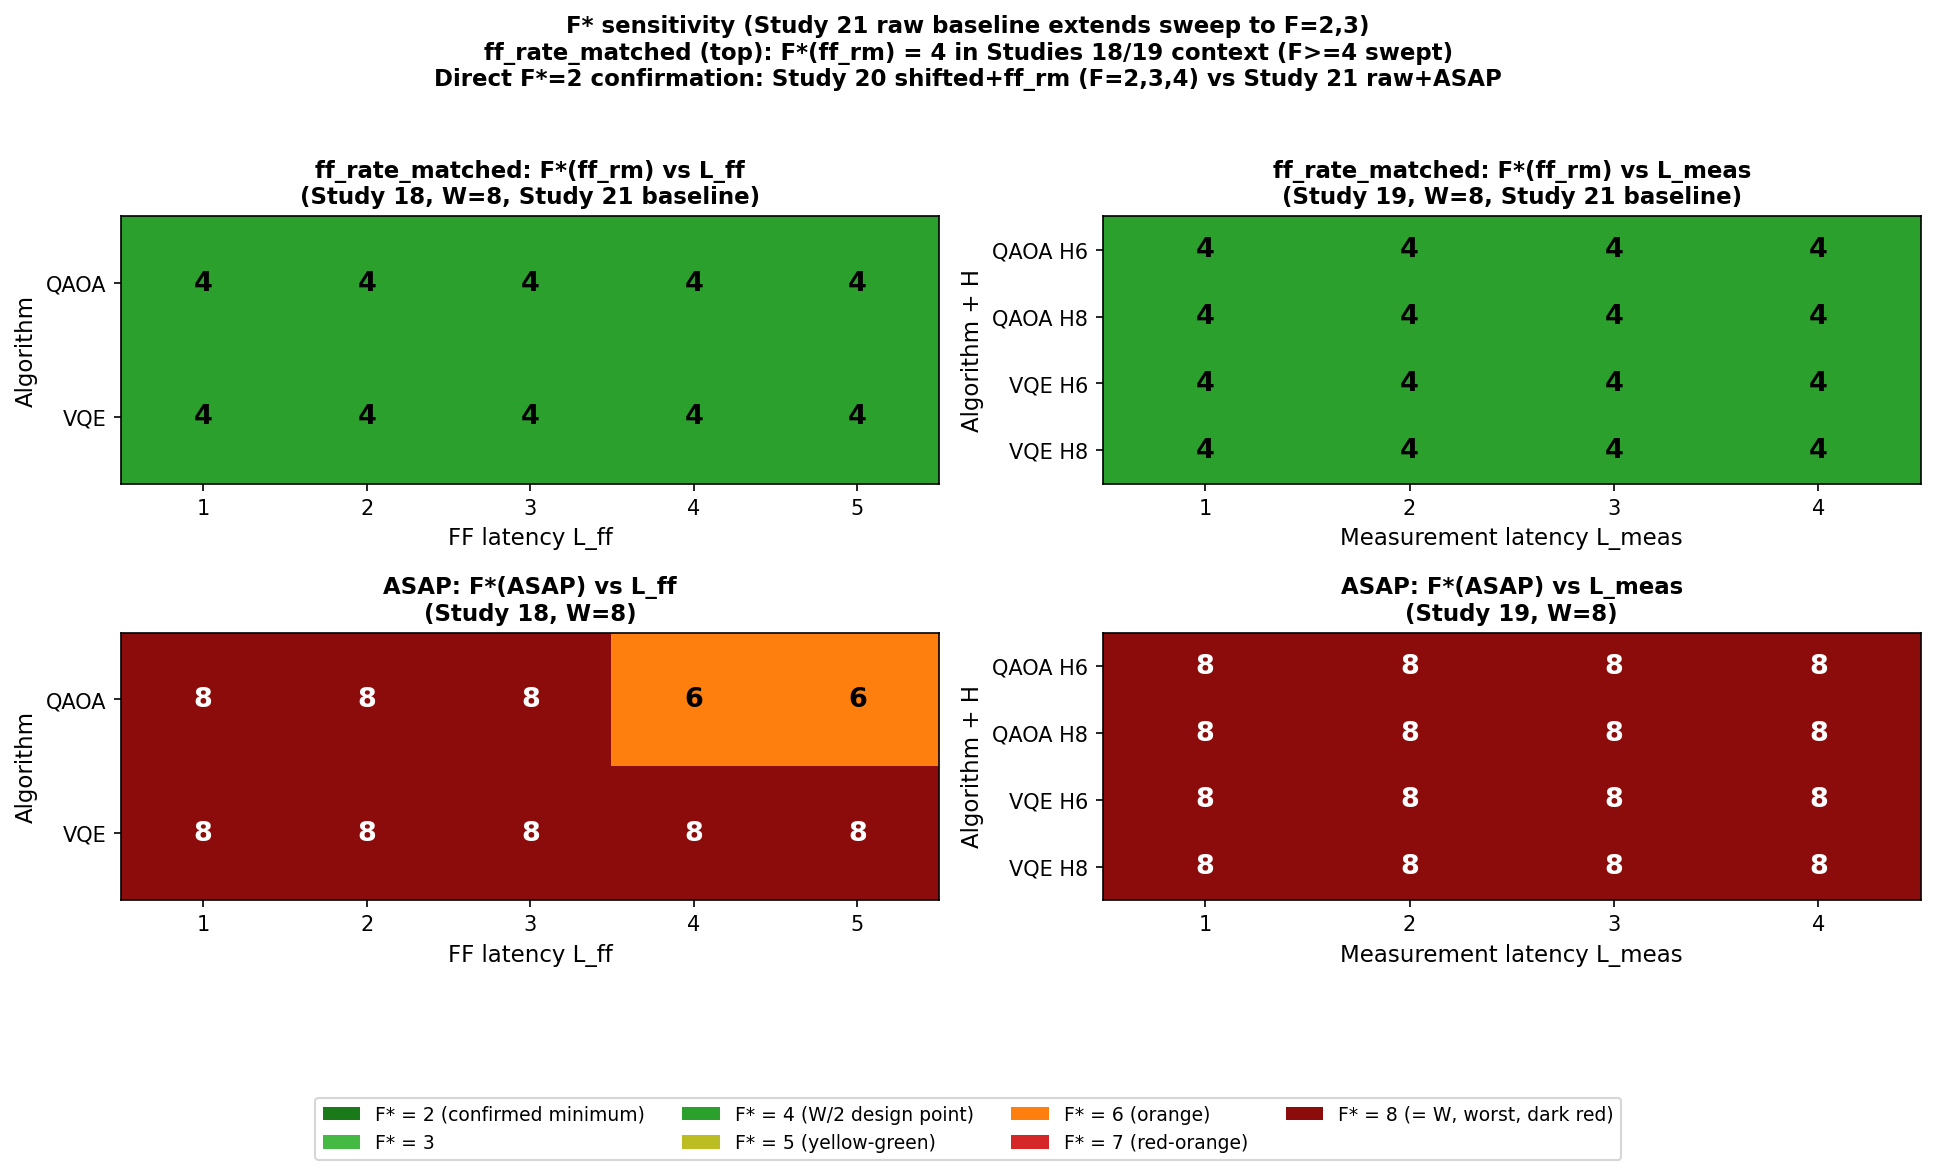
\includegraphics[width=\columnwidth]{figures/fig6_sensitivity.png}
  \caption{感度ヒートマップ：
  $F^*(\texttt{ff\_rate\_matched}) = 4 = W/2$ は
  $L_{\mathrm{ff}}$（左パネル）と $L_{\mathrm{meas}}$（右パネル）にわたって不変；
  $F^*(\text{ASAP})$ は 6〜8 に達する（下段）．
  上段の全セルが均一に緑（$F^*=4$）であることが中心的実証的主張である．}
  \label{fig:sensitivity}
\end{figure}

\begin{figure}[t]
  \centering
  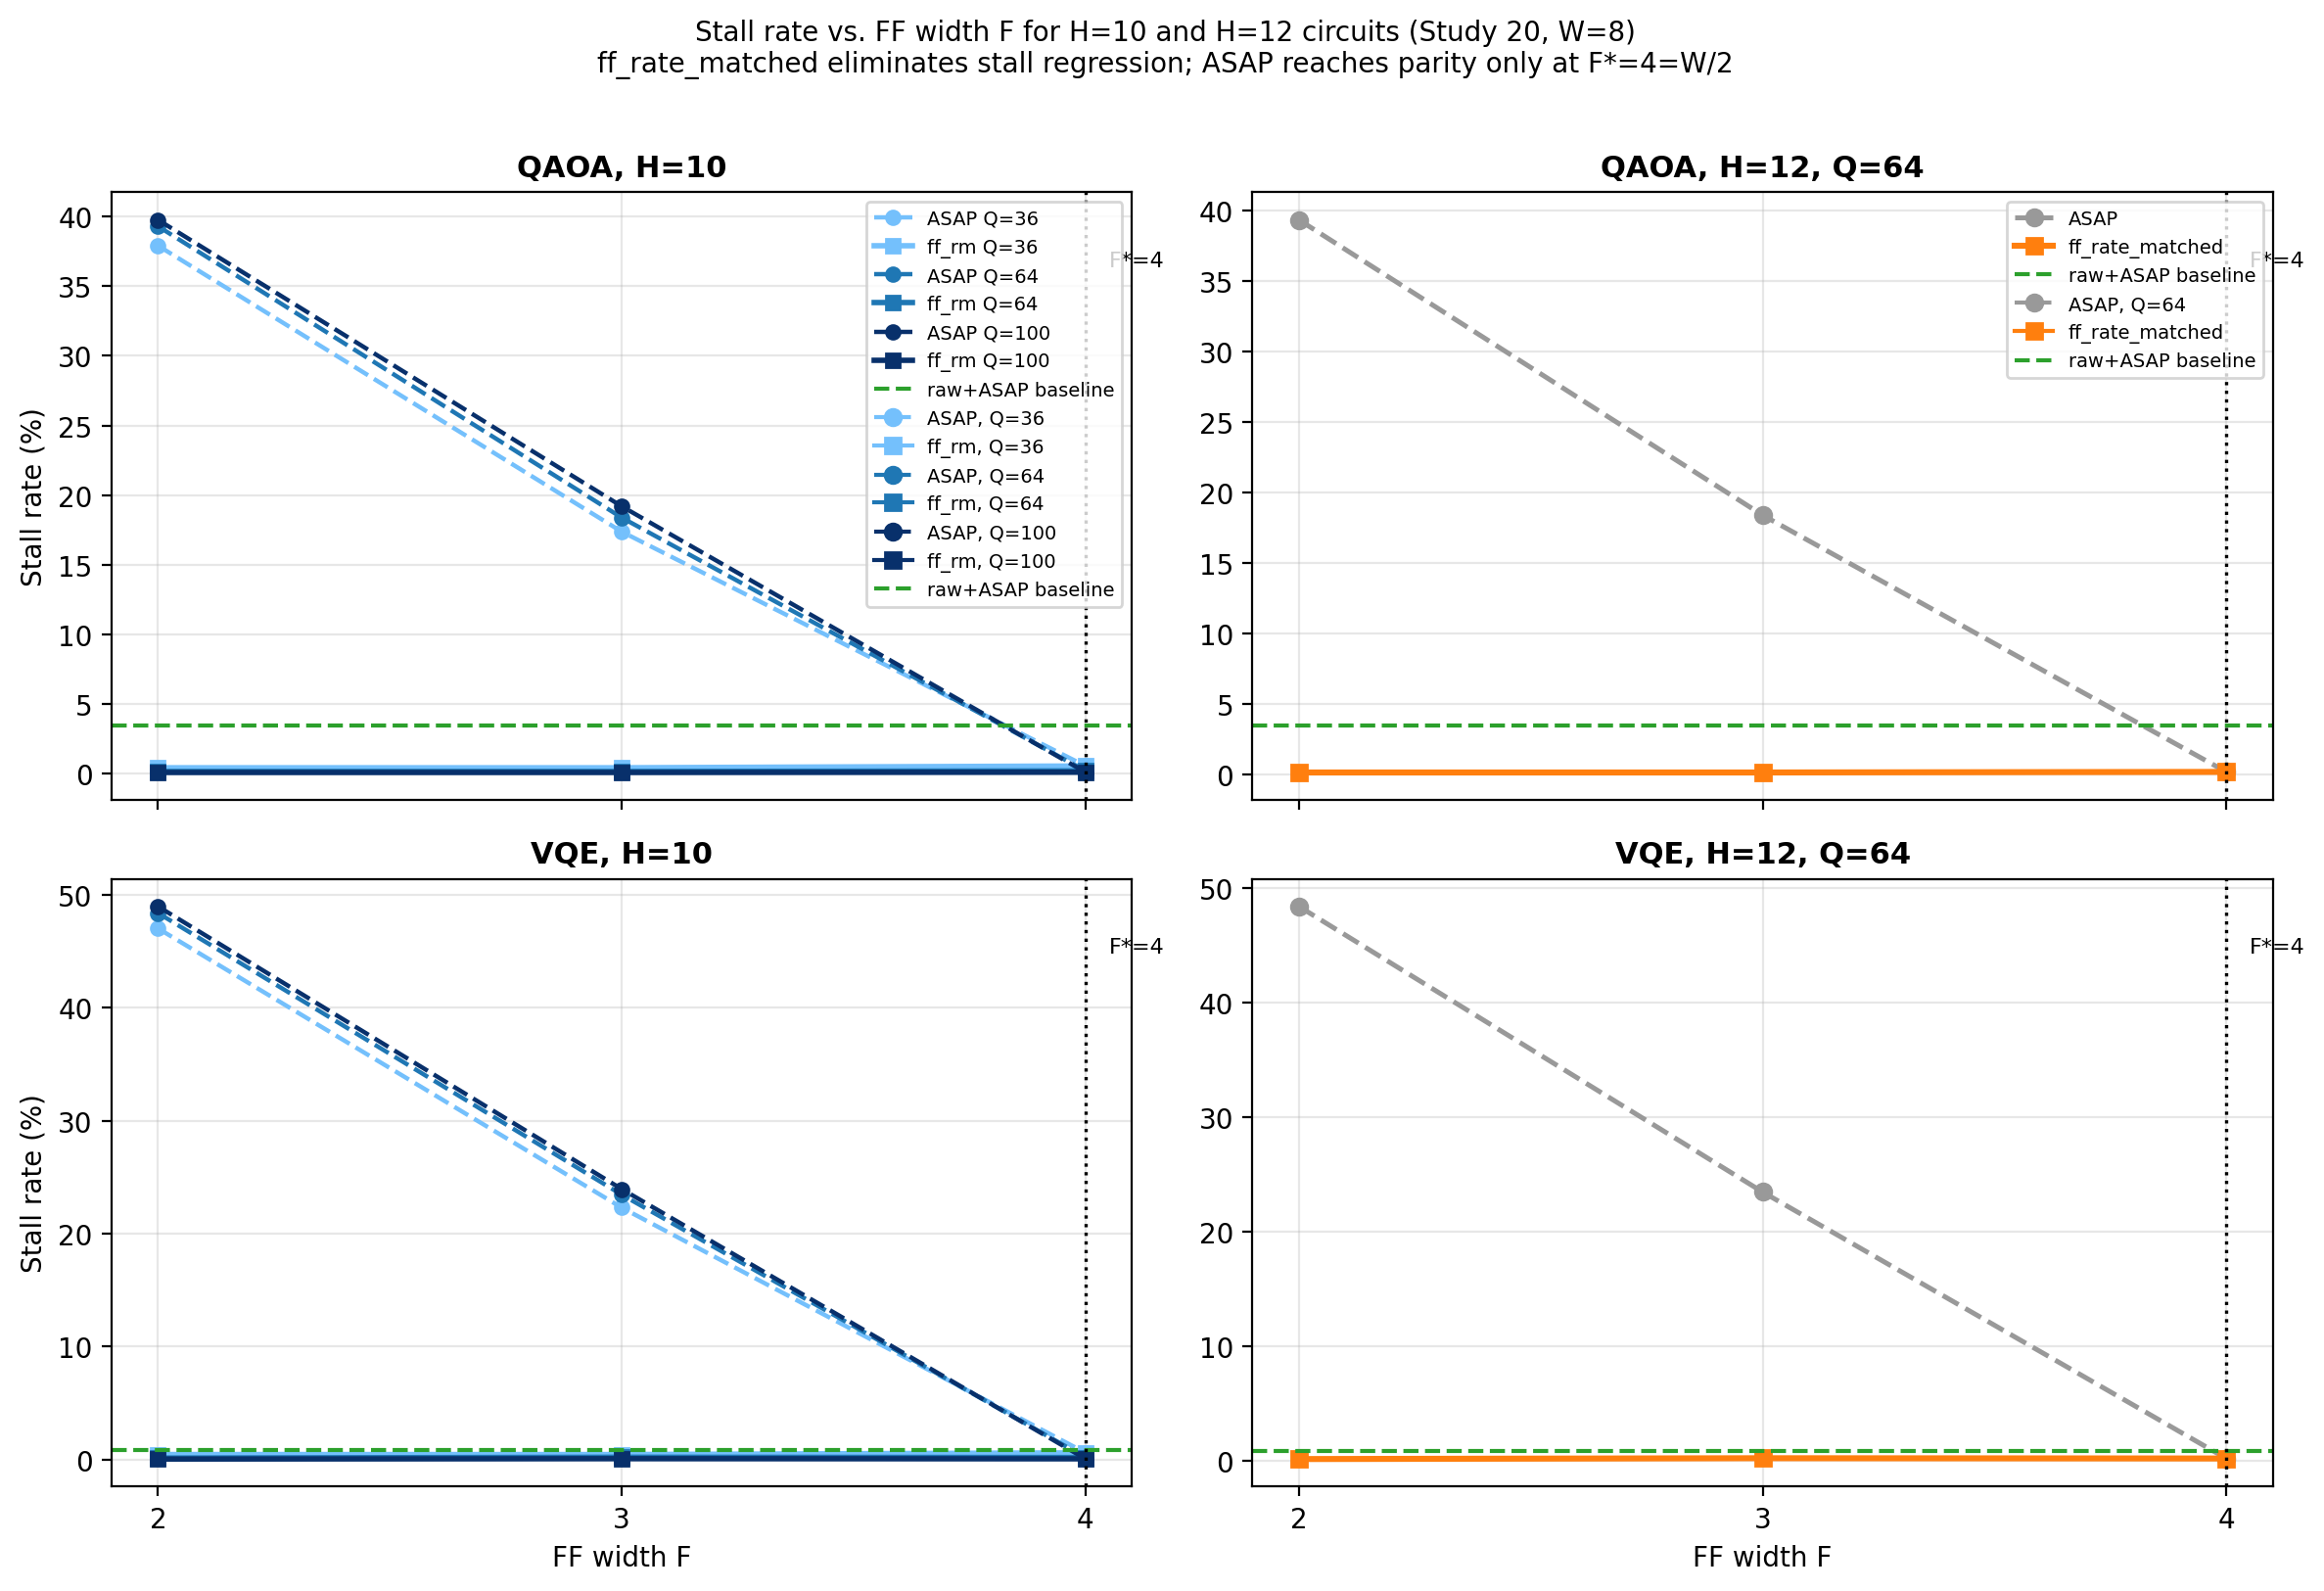
\includegraphics[width=\columnwidth]{figures/fig7_scaling.png}
  \caption{Study~20 ($W=8$) における FF 幅 $F$ の関数としてのストール率．
  上段：QAOA；下段：VQE．左列：H=10（Q=36, 64, 100）；右列：H=12, Q=64．
  縦点線が設計点 $F^* = W/2 = 4$ を示す．}
  \label{fig:scaling}
\end{figure}

\textbf{スループット結果．}
全 1,080 ペア比較で cycles\_ratio の中央値 = 1.000000，
完全サイクル一致 1,080/1,080 (100\%)，cycles\_ratio $> 1$ は 0 件．

\textbf{ストール率結果（代表例，$W=4$，$L_{\mathrm{meas}}=1$，$L_{\mathrm{ff}}=2$）：}

\begin{table}[h]
\centering
\caption{Study~20: ASAP vs. ff\_rate\_matched ストール率（$W=4$）}
\label{tab:study20-stall}
\begin{tabular}{llcccc}
\toprule
Alg. & H & Q & $W$ & $F$ & ASAP / ff\_rm ストール \\
\midrule
QAOA & 10 & 100 & 4 & 2 & \textbf{39.7\%} / 0.05\% \\
QAOA & 10 & 100 & 4 & 3 & \textbf{19.2\%} / 0.05\% \\
QAOA & 10 & 100 & 4 & 4 & 0.07\% / 0.07\% \\
QAOA & 12 &  64 & 4 & 2 & \textbf{38.8\%} / 0.12\% \\
VQE  & 10 & 100 & 4 & 2 & \textbf{49.0\%} / 0.06\% \\
VQE  & 10 & 100 & 4 & 3 & \textbf{23.9\%} / 0.09\% \\
VQE  & 10 & 100 & 4 & 4 & 0.08\% / 0.08\% \\
VQE  & 12 &  64 & 4 & 2 & \textbf{48.4\%} / 0.15\% \\
\bottomrule
\end{tabular}
\end{table}

図~\ref{fig:sensitivity} と図~\ref{fig:scaling} が詳細を示す．

\subsection{Study 21：生 DAG スイープを F=1, 2, 3 に拡張}

\textbf{動機．}
Studies~17〜20 には $F < 4$ での生+ASAP スイープが含まれておらず，
$F^*(\texttt{ff\_rate\_matched}) < W/2$ である可能性が未検討のままであった．

\textbf{設定．}
生 DAG スイープを $F \in \{1, 2, 3, 4\}$，ASAP・ff\_rate\_matched ポリシー，
$W \in \{4, 8, 16\}$，$L_{\mathrm{meas}}=1$，$L_{\mathrm{ff}}=2$ で実行．
QAOA・VQE 回路（$H \in \{4, 6, 8\}$，$Q \in \{16, 36, 64\}$，シード 0〜4）．
合計：1,080 実行．

\textbf{クロス Study $F^*$ 判定：}

\begin{table}[h]
\centering
\caption{Study~21: クロス Study $F^*$ 比較}
\label{tab:study21}
\begin{tabular}{ccccc}
\toprule
Alg. & $F$ & 生+ASAP [H8/Q64] & シフト+ff\_rm [H10/Q100]
  & $F^* \leq F$？ \\
\midrule
QAOA & 1 & 16.91\% & 0.075\% & \textbf{Yes} \\
QAOA & 2 &  5.52\% & 0.051\% & \textbf{Yes} \\
QAOA & 3 &  2.53\% & 0.051\% & \textbf{Yes} \\
VQE  & 1 &  4.61\% & 0.090\% & \textbf{Yes} \\
VQE  & 2 &  0.29\% & 0.060\% & \textbf{Yes} \\
VQE  & 3 &  0.51\% & 0.090\% & \textbf{Yes} \\
\bottomrule
\end{tabular}
\end{table}

$F=1$ での cycles\_ratio は QAOA・VQE ともに 1.000（スループットコストゼロ）．

\textbf{非単調なストール率値についての注意．}
VQE H8/Q64 の生+ASAP ストール率が $F$ とともに増加する（$F=2$: 0.29\%，
$F=3$: 0.51\%，$F=4$: 0.86\%）のは\textbf{分母効果}である．
VQE H8/Q64 は全シードで $D_{\mathrm{ff}}^{\mathrm{raw}} = 63$ を持ち，
total\_cycles は 2,058($F=2$) → 1,379($F=3$) → 1,043($F=4$) と急減するが，
stall\_cycles の絶対数は 6, 7, 9 とほぼ一定のため，
stall\_rate = stall\_cycles / total\_cycles が見かけ上増加する．

\subsection{実験結果の要約}

5 軸の検証により ff\_rate\_matched の実用的設計ガイドラインが確立される：

\begin{quote}
\textbf{ff\_rate\_matched は $F \leq W/2$ でストール回帰を除去し，
ほぼゼロのスループットコスト（1,440 中 1,430 の完全サイクル一致；
例外 10 件の QFT は $\leq 0.16\%$ の偏差）を達成する．
この保証は，$F/W \in [0.125, 1.0]$，$L_{\mathrm{ff}} \in [1, 5]$，
$L_{\mathrm{meas}} \in [1, 4]$，$H=12$・$Q=100$ までの回路規模にわたって
QAOA・VQE アルゴリズムで確認されている．}
\end{quote}

逆に ASAP は最悪のケース（大 $Q$ の VQE）で $F = W$ を必要とし，
FF ハードウェア要件を 2 倍にする．

% ============================================================
\section{関連研究}

\subsection{MBQC コンパイルと古典制御}

MBQC は Raussendorf と Briegel \cite{RaussendorfBriegel2001} によって導入され，
測定計算 \cite{DanosKashefi2006} がシグナルシフトを含む書き換えルールを
形式化した．
Broadbent と Kashefi \cite{Broadbent2009} は異なるコンパイル戦略下での
深さ複雑性を解析した．
古典制御レイテンシの重要性は誤り耐性量子計算の文脈
\cite{FowlerMartinis2012,RaussendorfHarrington2007} において指摘されている．

\subsection{オンチップネットワークにおけるフロー制御}

クレジットベースフロー制御は Dally と Towles \cite{DallyTowles2004} によって
体系化された．
Kumar ら \cite{KumarPeh2007} は NoC ルーターにおけるバースト性トラフィックで
クレジットプールサイズがリンク帯域幅の半分で十分であることを示し，
私たちの $F^* = W/2$ の結果を補完的に裏付ける．

\subsection{スーパースカラ・ハザード検出}

RAW ハザードとの構造的類比 \cite{Tomasulo1967,HennessyPatterson2017} は
Section~\ref{sec:design} で述べた．
ff\_rate\_matched は個々の依存関係を追跡する代わりに
処理中の総数に上限を設ける，より単純な構造的ハザード防止を実装する．

\subsection{スケジューリング理論}

Little's Law \cite{Little1961} は $F^* = W/2$ に対する有用な一貫性チェックを
提供し，$\lambda \leq F / L_{\mathrm{ff}}$ の制限を導く．
RMS の利用率上限 \cite{LiuLayland1973} との類比は Section~IV-B で議論した．

% ============================================================
\section{考察}

\subsection{ハードウェアへの示唆}

本研究の中心的な実用的示唆は \textbf{FF ハードウェア要件の 50\% 削減}である．
$W = 16$ のシステムでは FF スロット数が 16 から 8 に削減される．
Study~21 はクロス Study 比較において最小実行可能 $F$ が 1 という低さで済む
可能性を示唆する（87.5\% の面積削減に相当）．

\subsection{シグナルシフトコンパイルとの関係}

本結果はシグナルシフトコンパイルの価値を損なうものではなく，むしろ補完する．
本研究から浮かび上がる co-design 原理は：

\begin{quote}
\textit{シグナルシフトコンパイルを適用する場合，ff\_rate\_matched スケジューリングと
組み合わせて $F = W/2$ を設定せよ．
これにより FF 回帰ゼロ・FF ハードウェア面積半分で
シグナルシフトの完全なスループット利益が得られる．}
\end{quote}

\subsection{限界と将来の研究}

\textbf{$D_{\mathrm{ff}} \leq 2$ を超える一般性．}
$H=8$，$Q=64$ の QFT は残留 $D_{\mathrm{ff}}^{\mathrm{shifted}} = 27$〜$31$ を示す
具体的な例であり，このような $D_{\mathrm{ff}} > 2$ のプログラムでは
$F^* = W/2$ の保証が再検討を要する．

\textbf{同一回路での $F^*=1$ 確認．}
Study~21 はクロス Study 比較で基準を確認したが，
同一回路での直接比較は将来の研究に委ねられる．

\textbf{適応的クレジットサイジング，確率的 FF レイテンシ，
誤り耐性 MBQC} など，さらなる拡張方向が存在する（Section~VII 参照）．

% ============================================================
\section{結論}

本論文では，シグナルシフトコンパイル下での MBQC 古典制御のためのクレジットベース
フィードフォワード幅スケジューリングポリシーである ff\_rate\_matched を提案した．
このポリシーはストール回帰問題を，発行-FF インターフェースでの
クレジットベースフロー制御の適用によって解決する．

主要な貢献は，$F^*(\texttt{ff\_rate\_matched}) \leq \lceil W/2 \rceil$ の
実証的に確認された設計原理であり，4,360+ 回のシミュレーション実行にわたる
5 軸の実験で確認されている：

\begin{itemize}
\item \textbf{スループットコスト}：ほぼゼロ――1,440 ペア中 1,430 ペアが同一
  総サイクル数，例外 10 件はすべて偏差 $\leq 0.16\%$ の QFT 回路．
\item \textbf{レイテンシロバスト性}：$F^* \leq W/2$ は $L_{\mathrm{ff}} = 1$〜$5$
  と $L_{\mathrm{meas}} = 1$〜$4$ にわたって不変（Studies~18, 19）．
\item \textbf{スケールロバスト性}：$H=12$，$Q=100$ で 1,080 の完全サイクル
  一致により確認（Study~20）．
\item \textbf{エンドツーエンド co-design}：シフト済み + ff\_rate\_matched は
  生 + ASAP より低い総サイクル数を達成（Section~V-C）．
\item \textbf{Study~21（F=1 拡張）}：クロス Study 比較で $F^*$ 基準が $F=1$
  において満たされ，$F=W/2$ は 4 倍の安全マージンを持つ保守的設計点．
  $F=1$ でスループットコストゼロを確認．
\end{itemize}

より広い視点では，本研究は古典コンピュータアーキテクチャ技術――
NoC 設計からのクレジットベースフロー制御，
スーパースカラ CPU からの RAW ハザード防止，
待ち行列理論からのフロー平衡解析――が
MBQC 古典制御領域に直接かつ生産的に移転できることを示す．
量子プロセッサがスケールし古典制御がますます支配的なコストとなるにつれて，
これらの学際的接続は MBQC システム設計の本質的なツールとなるだろう．

% ============================================================
\bibliographystyle{IEEEtran}
\begin{thebibliography}{99}

\bibitem{RaussendorfBriegel2001}
R.~Raussendorf and H.~J.~Briegel,
``A one-way quantum computer,''
\emph{Physical Review Letters}, vol.~86, no.~22, pp.~5188--5191, 2001.

\bibitem{RaussendorfBrowne2003}
R.~Raussendorf, D.~E.~Browne, and H.~J.~Briegel,
``Measurement-based quantum computation on cluster states,''
\emph{Physical Review A}, vol.~68, no.~2, p.~022312, 2003.

\bibitem{RaussendorfHarrington2007}
R.~Raussendorf and J.~Harrington,
``Fault-tolerant quantum computation with high threshold in two dimensions,''
\emph{Physical Review Letters}, vol.~98, no.~19, p.~190504, 2007.

\bibitem{DanosKashefi2006}
V.~Danos and E.~Kashefi,
``Determinism in the one-way model,''
\emph{Physical Review A}, vol.~74, no.~5, p.~052310, 2006.

\bibitem{Broadbent2009}
A.~Broadbent and E.~Kashefi,
``Parallelizing quantum circuits,''
\emph{Theoretical Computer Science}, vol.~410, nos.~26--28,
pp.~2489--2510, 2009.

\bibitem{DallyTowles2004}
W.~J.~Dally and B.~Towles,
\emph{Principles and Practices of Interconnection Networks}.
Morgan Kaufmann, 2004.

\bibitem{KumarPeh2007}
A.~Kumar, L.-S.~Peh, and N.~K.~Jha,
``Token flow control,''
in \emph{Proc. 40th IEEE/ACM Int. Symp. Microarchitecture (MICRO-40)},
pp.~342--353, 2007.

\bibitem{Tomasulo1967}
R.~M.~Tomasulo,
``An efficient algorithm for exploiting multiple arithmetic units,''
\emph{IBM Journal of Research and Development}, vol.~11, no.~1,
pp.~25--33, 1967.

\bibitem{HennessyPatterson2017}
J.~L.~Hennessy and D.~A.~Patterson,
\emph{Computer Architecture: A Quantitative Approach}, 6th~ed.
Morgan Kaufmann, 2017.

\bibitem{Little1961}
J.~D.~C.~Little,
``A proof for the queuing formula: $L = \lambda W$,''
\emph{Operations Research}, vol.~9, no.~3, pp.~383--387, 1961.

\bibitem{LiuLayland1973}
C.~L.~Liu and J.~W.~Layland,
``Scheduling algorithms for multiprogramming in a hard-real-time environment,''
\emph{Journal of the ACM}, vol.~20, no.~1, pp.~46--61, 1973.

\bibitem{FowlerMartinis2012}
A.~G.~Fowler, M.~Mariantoni, J.~M.~Martinis, and A.~N.~Cleland,
``Surface codes: Towards practical large-scale quantum computation,''
\emph{Physical Review A}, vol.~86, no.~3, p.~032324, 2012.

\bibitem{DelfosseNickerson2021}
N.~Delfosse and N.~H.~Nickerson,
``Almost-linear time decoding algorithm for topological codes,''
\emph{Quantum}, vol.~5, p.~595, 2021.

\end{thebibliography}

\end{document}
